%%%%%%%%%%%%%%%%%%%%%%%%%%%%%%%%%%%%%%%%%%%%%%%%%%%%%%%%%%%%%%%%%
% Lecture date: 19-12-09
%%%%%%%%%%%%%%%%%%%%%%%%%%%%%%%%%%%%%%%%%%%%%%%%%%%%%%%%%%%%%%%%%
\chapter{Electroweak Processes}
We will consider $\SU(2)_\text{L} \times \Uni(1)_\text{Y}$ theory.

\section{Muon decay}
$V-A$ interaction

\begin{align*}
   \feynmandiagram[horizontal=i1 to v1, medium, layered layout]{
      i1[particle=\(\mu\)] --[momentum=\(p\), fermion]v1,
      v1 --[momentum=\(k_1\), fermion] f3[particle=\(\nu_\mu\)],
      v1 -- [photon, edge label=\(W\)] v2,
      {[same layer] v2, f3},
      v2 --[fermion, momentum=\(k_2\)] f1[particle=\(e^-\)],
      v2 --[anti fermion, momentum=\(k_3\)] f2[particle=\(\bar\nu_e\)],
      {[same layer] f1, f2},
   };
\end{align*}

$q = k_2 + k_3 = p - k_1$
\begin{align*}
   i \M = \overline{u}(k_1)  \frac{-ig}{\sqrt{2}} \gamma^\mu P_L u(p) \frac{-ig_{\mu\nu}}{q^2 - M_W^2} \overline{u}(k_2) \frac{-ig}{\sqrt{2}} \gamma^\nu P_L v(k_3)
\end{align*}

In spinor space, Dirac equation 
\begin{align}
   (\slashed{p} - m) u(p) = 0.
\end{align}

Propagator $M_W \sim \SI{80}{\giga\eV}$ and $m_\mu = \SI{100}{\mega\eV}$, i.e.~$p^2 \ll M^2$. So $4$-Fermi approximation is obtained.
\begin{align*}
   \frac{1}{q^2 - M_W^2} = - \frac{1}{M_W^2} \frac{1}{1 - q^2 / M_W^2} \approx -\frac{1}{M_W^2}
\end{align*}
Then the coupling is effectively
\begin{align}
   G_F = \frac{\sqrt{2} g^2}{8 M_W^2}
\end{align}
Note that when for example top and bottom quarks are present, this approximation is not valid any more.

Proceed with $m_e = m_{\nu_e} = m_{\nu_\mu} = 0$
\begin{align*}
   \M &= -\frac{4G_F}{\sqrt{2}} \overline{u}(k_1) \gamma^\mu P_L u(p) \overline{u}(k_2) \gamma_\mu P_L v(k_3) \\
   \frac{1}{2} \sum_{\text{spins}} |\M|^2 &= \frac{16 G_F^2}{2 \cdot 2} \overline{u}(k_1) \gamma^\mu P_L u(p) \overline{u}(p) P_R \gamma^\nu u(k_1) \overline{u}(k_2) \gamma_\mu P_L v(k_3) \overline{v}(k_3) P_R \gamma_\nu u(k_2) \\
                                          &= 4 G_F^2 \tr[\slashed{k}_1 \gamma^\mu P_L (\slashed{p} + m_\mu) P_R \gamma^\nu] \cdot \tr[\slashed{k}_2 \gamma_\mu P_L \slashed{k}_3 P_R \gamma_\nu]
                                          \shortintertext{Term with $m_\mu$ vanishes, since $P_L P_R = 0$}
\end{align*}

Computing the two traces
\begin{align*}
   \tr[\slashed{k}_1 \gamma^\mu \slashed{p}\gamma^\nu P_L] &= \frac{4}{2}  \left( k_1^\mu p^\nu - k_1 p g^{\mu\nu} + k_1^\nu p^\mu \right) - \frac{4i}{2} \epsilon_{\alpha\mu\beta \nu} {k_1}_\alpha p_\beta  \\
   \tr[\slashed{k}_2 \gamma_\mu \slashed{k}_3 \gamma_\nu P_L] &= \frac{4}{2}  \left( (k_2)_\mu (k_3)_\nu - k_2 k_3 g_{\mu\nu} + {k_2}_\nu {k_3}_\mu \right) + \frac{4i}{2} \epsilon \epsilon_{\alpha \mu \beta \nu} k_2^\alpha k_3^\beta
\end{align*}
Using the fact that $\epsilon$ is totally anti-symmetric tensor, so the terms with one $\epsilon$ sum to zero. Note further
\begin{align}
   \epsilon^{\mu\nu\rho\sigma} \epsilon_{\mu\nu}^{\quad \rho'\sigma'} = -2 (g^{\rho \rho'}g^{\sigma \sigma'} - g^{\rho\sigma'} g^{\rho'\sigma})
\end{align}

In order to use this formula
\begin{align*}
   &\sigma^{\alpha \mu \beta \nu} \sigma_{\alpha' \mu \beta' \nu} \\
   &= \epsilon^{\mu \nu \alpha \beta} \epsilon^{\quad \alpha'' \beta''}_{\mu\nu} g_{\alpha' \alpha ''} g_{\beta ' \beta''} \\
   &= (-2) \left[ g^{\alpha \alpha''} g^{\beta \beta''} - g^{\alpha \beta''} g^{\beta \alpha''}\right] g_{\alpha' \alpha''} g_{\beta' \beta''} \\
   &= (-2) \left[ \delta^{\alpha}_{\alpha'} \delta^{\beta}_{\beta'} - \delta^{\alpha}_{\beta'} \delta^{\beta}_{\alpha'}  \right]
\end{align*}

Terms without $\epsilon$
\begin{align*}
   &4 (k_1^\mu p^\nu + k_1^\nu p^\mu - g^{\mu\nu} k_1 \cdot p) (k_{2 \mu} k_{3 \nu} + k_{2\nu} k_{3\mu} - k_2 \cdot k_3 g_{\mu\nu}) \\
   &= \dots = 4 \left[ 2 (k_1 \cdot k_2) (p\cdot k_3) + 2 (k_1\cdot k_3)( p \cdot k_2) \right] \\
   &= 8 \left[ (k_1 \cdot k_2)( p \cdot k_3) + (k_1 \cdot k_3) (p \cdot k_2) \right]
\end{align*}

Then
\begin{align*}
   \frac{1}{2} \sum_{\text{spins}} |\M|^2 = 64 G_F^2 (k_1 \cdot k_2)( p\cdot k_3)
\end{align*}
Recall
\begin{align}
   \begin{split}
   \dd{\Gamma} &= \frac{1}{2E} \overline{|\M|^2} \dd{Q} \\
   \dd{Q} &= \frac{\dd[3]{k_1}}{(2\pi)^3 2 E_{k_1}} \frac{\dd[3]{k_2}}{(2\pi)^3 2 E_{k_2}} \frac{\dd[3]{k_3}}{(2\pi)^3 2 E_{k_3}} (2\pi)^{4} \delta^{(4)} (p-k_1 -k_2 - k_3)
   \end{split}
\end{align}

One can prove (In \sm neutrino has no mass.)
\begin{align}
   \frac{\dd[3]{k_1}}{(2\pi)^3 2 E_{k_1}} = \int \dd[4]{k_1} \theta(E_1) \delta(k_1^2)
\end{align}

Use identity of Delta function involving composite function.
\begin{align*}
   \frac{\dd[3]{k_1}}{(2\pi)^3 2 E_{k_1}} \delta^{(4)}(p- k_1 -k_2 - k_3 ) = \int \dd[4]{k_1} \theta(E_1) \delta(k_1^2) \delta^{(4)}(p- k_1 -k_2 - k_3 ) \\
   = \theta(k_1)\delta^{k_1^2}
\end{align*}

Thus 
\begin{align*}
   \dd{Q} = \frac{1}{(2\pi)^5} \frac{\dd[3]{k_2}}{2E_{k_2}} \frac{\dd[3]{k_3}}{2E_{k_3}} \theta(E - E_{k_2} - E_{k_3}) \delta((p-k_2-k_3)^2)
\end{align*}

In rest frame of muon 
$p \cdot k_3 = m_\mu \cdot E_3$
\begin{align*}
   (k_1 + k_2)^2 &\approx 2 k_1 \cdot k_2 \\
   k_1 \cdot k_2 &\approx \frac{1}{2} (k_1 + k_2)^2 \\
                 &= \frac{1}{2} (p-k_3)^2 \\
                  &= \frac{1}{2} \left[ p^2 - 2 p\cdot k_3 + k_3^2 \right] \\
                  &= \frac{1}{2} [m_\mu^2 - 2 m_\mu E_3]
\end{align*}

\begin{align*}
   \frac{1}{2} \overline{|\M|^2} &= 64 G_F^2 k_1\cdot k_2 p \cdot k_3 \\
   &= 64 G_F^2 m_\mu E_3 [m_\mu^2 - 2 m_\mu E_3]
\end{align*}
Now we have computed $|\M|^2$, the actual difficulties are in phase space integral. For $n$-particle phase space, often use Monte-Carlo integration technique.

With $\theta$ the angle between electron and electron neutrino ($k_2$ and $k_3$)
\begin{align*}
   (p-k_2 - k_3)^2 = p^2 + k_2^2 + k_3^2 - 2 p \cdot k_2 -2 p\cdot k_3 + 2k_2 \cdot k_3 \\
   = m_\mu^2 - 2 m_\mu E_2 - 2m_\mu E_3 + 2 E_2 E_3 (1-\cos \theta)
\end{align*}

\begin{align*}
   \dd[3]{k_2} \dd[3]{k_3} = (4\pi) (2\pi) E_2^2 \dd{E_2} E_3^2 \dd{E_3} \dd{\cos \theta}
\end{align*}

\begin{align*}
   \delta(\dots - 2 E_2 E_3 \cos \theta) = \frac{1}{2E_2 E_3} \delta(- \cos \theta)
\end{align*}

\begin{align*}
   \dd{\Gamma} = \frac{G_F^2}{2 \pi^3} \dd{E_3} \dd{E_3} E_3 (m_\mu^2 - 2 m_\mu E_3)
\end{align*}

\begin{align*}
   \frac{1}{2} m_\mu - E_2 \leq E_3 \leq \frac{1}{2} m_\mu \\
   0 \leq E_2 \leq \frac{1}{2} m_\mu
\end{align*}

Carrying the integration out
\begin{align*}
   \frac{\dd{\Gamma}}{\dd{E_2}} &= \frac{m_\mu G_F^2}{2\pi^3} \int_{\frac{1}{2}m_\mu - E_2}^{\frac{1}{2}m_\mu} \dd{E_3} E_3 (m_\mu - 2 E_3) \\
                                &= \frac{G_F^2}{2\pi^3} m_\mu^2 E_2^2 \left( 3 - \frac{4E_2}{m_\mu} \right)
\end{align*}

Finally
\begin{align*}
   \Gamma = \frac{1}{\tau_\mu} = \int^{\frac{1}{2}m_\mu}_0 \dd{E_2} \frac{\dd{\Gamma}}{\dd{E_2}} = \frac{G_F^2 m_\mu^5}{192 \pi^3}
\end{align*}
If $m_e \neq 0$
\begin{align*}
   \Gamma = \frac{1}{\tau_\mu} = \int^{\frac{1}{2}m_\mu}_0 \dd{E_2} \frac{\dd{\Gamma}}{\dd{E_2}} = \frac{G_F^2 m_\mu^5}{192 \pi^3} \left[ 1 - 8r^2 + 8r^6 - r^8 - 24 r^4 \ln{r} \right]
\end{align*}
with $r = m_e / m_\mu$. $r$ enters in boundary of phase space integration.
%%%%%%%%%%%%%%%%%%%%%%%%%%%%%%%%%%%%%%%%%%%%%%%%%%%%%%%%%%%%%%%%%
% Lecture date: 19-12-16
%%%%%%%%%%%%%%%%%%%%%%%%%%%%%%%%%%%%%%%%%%%%%%%%%%%%%%%%%%%%%%%%%

If one tries to measure the decay width precisely, the $1$-loop electroweak correction must also be included.
%TODO: diagram
\begin{align*}
   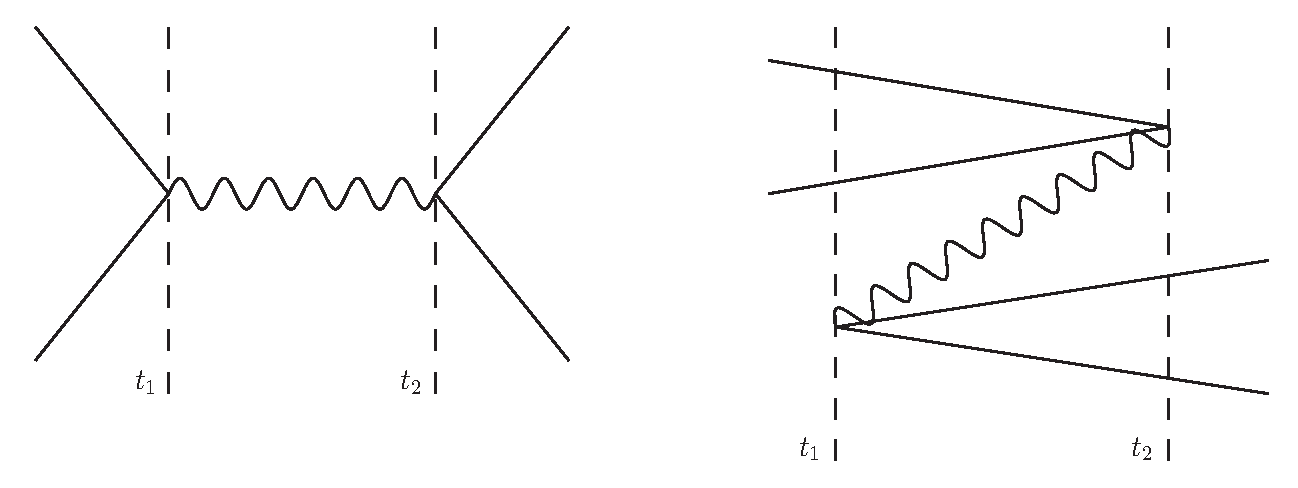
\includegraphics[width=0.5\linewidth]{muonDecay/1.eps}
\end{align*}

Neutrino can also be considered in the calculation and one finds an upper bound for neutrino mass $m_{\nu_\mu} \leq \SI{1}{\kilo \eV}$.

Mass dimension of $\Gamma$ is $+1$. Using dimensional argument, since $[G_F] = -2$, the decay width $\Gamma \sim G_F^2 m_\mu^5$. Grand Unified Theory postulates the decay of proton, $p \rightarrow e^+ \pi^0$. Following $M_{X,Y} \sim \SI{10e16}{\giga \eV}$, we estimate the decay width of proton $\Gamma \sim \frac{g_{\mathbf{SU}(5)}^4}{M_X^4} M^5_{p}$.
\begin{align*}
   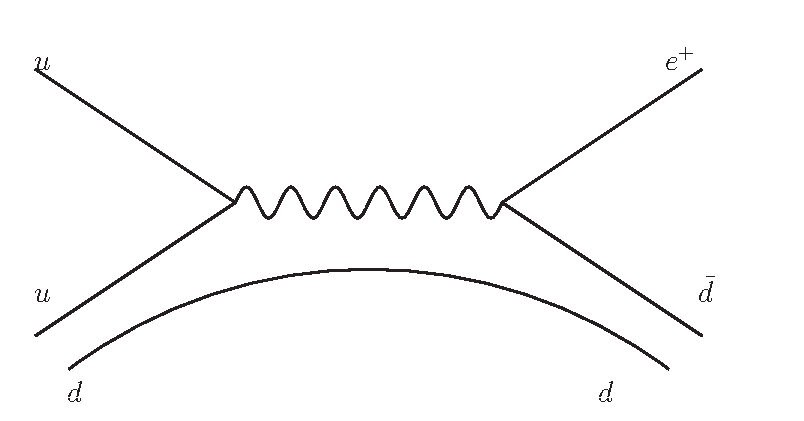
\includegraphics[width=0.5\linewidth]{muonDecay/2.eps}
\end{align*}

\paragraph{Polarized Muon Decay}
In the above computation, the muon polarizations are summed over. Assume the polarization is fixed
% TODO: diagram. helicity and angular momentum conservation

Also the spin sum relation enables us the computation. How to compute decay of polarized particle then? Recall that $u$, $\bar{u}$, $v$ and $\bar{v}$ are independent solutions to Dirac equation.
\begin{align}
   u^{(s)} = \sqrt{E+m} \begin{pmatrix} \chi^{(s)} \\ \frac{\pmb{\sigma} \cdot \pmb{p}}{E+m} \chi^{(s)} \end{pmatrix}
\end{align}
To get chiral-left part of $u^{(s)}$ $P_L u^{(s)}(\pmb{p})$. Can also define two projection operators
\begin{align}
   \Lambda_+ &= \frac{1}{2m} (\slashed{p} + m) \\
   \Lambda_- &= \frac{1}{2m} (-\slashed{p} + m)
\end{align}

They are indeed projection operators
\begin{align*}
   \Lambda_+ + \Lambda_- &= \id_4 \\
   (\Lambda_+)^2 &= \frac{1}{4m^2} \left( \slashed{p} \slashed{p} + 2m \slashed{p} + m^2 \right) = \frac{1}{4m^2} 2m (\slashed{p} + m) = \Lambda_+ \\
   (\Lambda_-)^2 &= \Lambda_-
\end{align*}

Let $\sum_{r=1}^{4} a_r u^{(r)}$ be an arbitrary spinor
\begin{align*}
   \Lambda_+ &= \sum_{r=1}^{4} a_r u^{(r)} \\
             &= \sum_{r=1}^{4} a_r \left( \sum_{s=1}^{2} \frac{u^{(s)}\bar{u}^{(s)}}{2m} \right) u^{(r)}
   \shortintertext{use $\bar{u}^{(s)} u^{(r)} = 2m \delta^{rs}$}
             &= \sum_{r=1}^2 a_r u^{(r)}
\end{align*}
arbitrary $E > 0$ spinor. Thus $\Lambda_+$ projects to $E > 0$ states and $\Lambda_-$ projects $E<0$ states.

Particle at rest, spin $\pmb{s}$ and $|\pmb{s}|=1$. Write a four-vector $s^\mu = (0, \pmb{s})$. At rest $p^\mu = (m, 0)$ and $(s\cdot p) = 0$. 

Starting from the $s^\mu$, can compute $s'^\mu$ in any frame by a Lorentz boost.
\begin{align*}
   s^0 &= \frac{\pmb{p} \cdot \pmb{\xi}}{m} \\
   s^i &= \xi^i + \frac{(\pmb{p} \cdot \pmb{\xi})}{m(m+E)}p^i
\end{align*}
$\pmb{\xi}$ denotes the direction of spin and $|\pmb{\xi}| = 1$

Compute $s \cdot p$ in new frame
\begin{align*}
   s \cdot p &= \frac{\pmb{p} \cdot \pmb{\xi}}{m} E - \pmb{p} \cdot \pmb{\xi} \\
             &= \frac{\pmb{p}\cdot \pmb{\xi} \pmb{p}^2}{m (m+E)} \\
             &= \pmb{p} \cdot \pmb{\xi} \left[ \frac{E}{m} - 1 - \frac{\pmb{p}^2}{m(m+E)} \right] \\
             &=\frac{\pmb{p} \cdot \pmb{\xi}}{ m(m+E)}  \left[ E (m+E) - m(m+E) - \pmb{p}^2 \right] \\
             &= 0
\end{align*} 

Define two projection operators
\begin{align*}
   \Sigma_{\pm} &= \frac{1}{2} \left( \id_4 \pm \gamma^5 \slashed{s} \right) \\
   \Sigma_+ + \Sigma_- &= \id_4 \\
   (\Sigma_-)^2 &= \frac{1}{4} (\id - \gamma^5 \slashed{s}) (\id - \gamma^5 \slashed{s}) \\
                &= \frac{1}{4} \left[ \id - 2 \gamma^5 \slashed{s} + \gamma^5 \slashed{s} \gamma^5 \slashed{s} \right]  \\
                &= \frac{1}{4} [ 2 \id - 2 \gamma^5 \slashed{s}] \\
                &= \Sigma_- \\
   (\Sigma_+)^2 &= \Sigma_+
\end{align*}

What do $\Sigma_\pm$ project out? In rest frame $\Sigma_- = \frac{1}{2} (\id - \gamma^5 \gamma^i s^i)$. Choose $\pmb{s} = \pmb{e}_3 = \pmb{e}_z$. 
\begin{align*}
   \Sigma_- &= \frac{1}{2} (\id - \gamma^5 \gamma^3) \\
            &= \frac{1}{2} \left[ \begin{pmatrix} \id_2 & 0 \\ 0 & \id_2\end{pmatrix}  - \begin{pmatrix} 0 &\id \\ \id & 0 \end{pmatrix} \begin{pmatrix} 0 & \sigma^3 \\ -\sigma^3 & 0 \end{pmatrix}\right] \\
            &= \frac{1}{2} \begin{pmatrix} \id_2 - \sigma^3 & 0 \\ 0 & \id_2 + \sigma^3 \end{pmatrix}
\end{align*}
so project out helicity states.

\begin{align}
   u^k(\pmb{p},s) \bar{u}_i ( \pmb{p}, s) = \frac{1}{2} \left[ (\slashed{p}+ m) (\id - \gamma^5 \slashed{s}) \right]_i^k
\end{align}
or in computation
\begin{align}
   (\slashed{p} + m ) \mapsto \frac{1}{2} (\slashed{p} + m_\mu) (\id - \gamma^5 \slashed{s}_\mu)
\end{align}

Turns out we can skip computation. Replace $p_\alpha \mapsto p_\alpha- m s_\alpha$ in final answer
\begin{align*}
   &\tr[\dots P_R (\slashed{p} + m_\mu) (\id -\gamma^5 \slashed{s}) \gamma_\alpha P_R \dots ] \\
   &= \tr \left[ \dots P_R (\slashed{p} - m_\mu \gamma^5 \slashed{s}) \gamma_\alpha P_R \dots \right] \\
   &= \tr \left[ \dots P_R (\slashed{p} - m \slashed{s}) \gamma_\alpha P_R \right]
\end{align*}
with
\begin{align*}
   \pmb{\xi} \cdot \frac{\pmb{p}_e}{|\pmb{p}_e|} = \cos \theta
\end{align*}
In the end
\begin{align}
   \frac{\dd{\Gamma}}{\Gamma} = \frac{1}{2} \left(1-\frac{1}{3}\cos \theta \right) \dd{\cos \theta}
\end{align}

\paragraph{Nuclear $\beta$-decay}
${}^{14}O \rightarrow {}^{14}N^* e^+ \nu_e$ $\beta^+$-emitter
$n \rightarrow p e^- \bar{\nu}_e$

Non-relativistic limit of Pauli-Dirac spinor
\begin{align*}
   u^{(s)}(\pmb{p}) &= \sqrt{E+m} \begin{pmatrix} \chi^{(s)} \\ \frac{\pmb{\sigma}\cdot \pmb{p}}{E + m} \chi^{(s)}\end{pmatrix} \\
   &\rightarrow \sqrt{2m} \begin{pmatrix} \chi^{(s)} \\ 0 \end{pmatrix}\\
   \bar{u}^{(s)} &= \sqrt{2m} \begin{pmatrix} x^{(s)} & 0\end{pmatrix}
\end{align*}

\begin{align*}
   &\bar{\psi}_n \gamma_\mu \frac{1}{2} \left( \id - \gamma^5 \right) \psi_p (x)
   \shortintertext{$\gamma^5$ matrice has no effect and vanishes}
   &= \frac{1}{2} \bar{\psi}_n (x) \gamma_\mu \psi_p (x) \\
   &= \frac{1}{2} \psi_n (x) \gamma^0 \gamma_\mu \psi_p (x) \\ 
   &\rightarrow  \frac{1}{2} \psi_n^\dagger \psi_p
\end{align*}

$\mu \rightarrow i=1,2,3$
\begin{align*}
   \gamma^0 \gamma^i &= \begin{pmatrix} \id_2 & 0 \\ 0 & -\id_2 \end{pmatrix} \begin{pmatrix} 0 & \sigma_i \\ -\sigma_i & 0 \end{pmatrix}\\
   &= \begin{pmatrix} 0 & \sigma_i \\ \sigma_i & 0 \end{pmatrix}
\end{align*}
It is off-diagonal.

Thus in the non-relativistic limit
\begin{align*}
   \psi_n&^\dagger \gamma^0 \gamma^i \psi_p \rightarrow 0
\end{align*}
